After shipping Wolfenstein 3D in May 1992, id Software went right back to work. The team of five (John Carmack, John Romero, Adrian Carmack, Tom Hall and Kevin Cloud) split in two. While part of the team would focus on Wolfenstein 3D Hint Manual and Spear of Destiny an other faction built the technology while would power the next title.\\
\par
The development of \doom~really start in January 1993 with an impressive press release by Tom Hall\protect\footnote{Annexe, p \ref{label_pressrelease}} promising ground-breaking technology and unprecedented gameplay. Within just eleven months they managed to have the shareware version ready in time for Christmas. No less than thirteen person would end up being involved.\\
\par
 \begin{figure}[H]
\centering  
\begin{tabularx}{\textwidth}{ X  X  X  }
  \toprule
  \textbf{Name} &  \textbf{Age} & \textbf{Occupation} \\
  \toprule 
   John Carmack & 22 &  Programming\\
   John Romero & 26 &  Programming\\
   Adrian Carmack & 23 &  Artist\\
   Tom Hall\protect\footnotemark  & 29 &  Creative Director\\
   Jay Wilbur & 31 &  Business\\
   Kevin Cloud& 28 &  Computer Artist\\
   Donna Jackson & 55 & id's Mom\\   
   Dave Taylor & 24 & Programming\\
   Sandy Petersen & 39 & Designer\\
   Shawn Green & 28 & Software Support\\
   American McGee & 22 & Tech Support\\
   Paul Radek & 28 & DMX Audio library\\
   Gregor Punchatz & 27 & Artist, clay models\\

     \toprule
\end{tabularx}
%\caption{Doom team}
\label{fig:Id Software team}
\end{figure}
\footnotetext{Due to creative differences, Tom Hall left the project shortly after completing the design doc "Doom Bible". He went to Apogee/3D Realms to work on "Rise of the Triad" using an improved version of Wolfenstein 3D engine.}



\par
\drawing{timeline}{Making of Doom timeline}
\par




% First good page in the whole book :) !
\fullimage{idsoftware_crew.png}

\begin{wrapfigure}[12]{r}{0.37\textwidth}
\scaledimage{0.37}{johns_weapons.png}
\end{wrapfigure}

In January of 1995, Electronic Games magazine ran a series of three articles for the release of Doom II. An opportunity to gather all members of id team in a group photo.\\
\par
 In the back row, left to right: Kevin~Cloud, American~Mcgee, John~Carmack, Adrian~Carmack, Sandy~Petersen. Front row , left to right: Dave~Taylor, John~Romero and Shawn~Green.\\
 \par The "plank" in the photo is John Romero's office door and the hole the making of John Carmack.\\
  \par
\fq{Well, Romero's doom jammed one day. He was in his office and was trapped in there,
and we couldn't get the door open. It was after-hours, so we couldn't call building
maintenance, and we were all standing around trying to figure out what to do, when
it occurred to me and I said, "You know, I do have a batle axe in my office."\\
\par
Yes, this thing really works.}{John Carmack}






\section{Location}
Fed up with the winter of Wisconscin, the studio relocated in November 1992. They left behind the cold of Madison and settled in the Town East Tower in Mesquite TX, better known as the "Black Cube".\\
\par
\bigskip
\begin{figure}[H]
\centering

\includegraphics[width=\textwidth]{drawings/usa-id-software.pdf}
\end{figure}
\par
\bigskip
In an interview for the book "Masters of Doom", Tom Halls remembered how all team members settled in the new environment.\\
\par
\fq{On the first day, each guy chose his space. Carmack and Romero took side-by-side offices, while Adrian and Kevin, who were growing increasingly close, decided to share a space. Tom liked an open corner spot in a large room with a window. "This would be a great office area," he said, "we just need to put some walls up." The rest agreed. But the walls were slow to come. When- ever Tom asked Jay about it, Jay would say they were on their way. Out of humor and frustration, Tom put down two long strips of masking tape where the walls of what he called his creative corner would go.}{David Kushner, Masters of Doom}
\par
\begin{figure}[H]
\centering
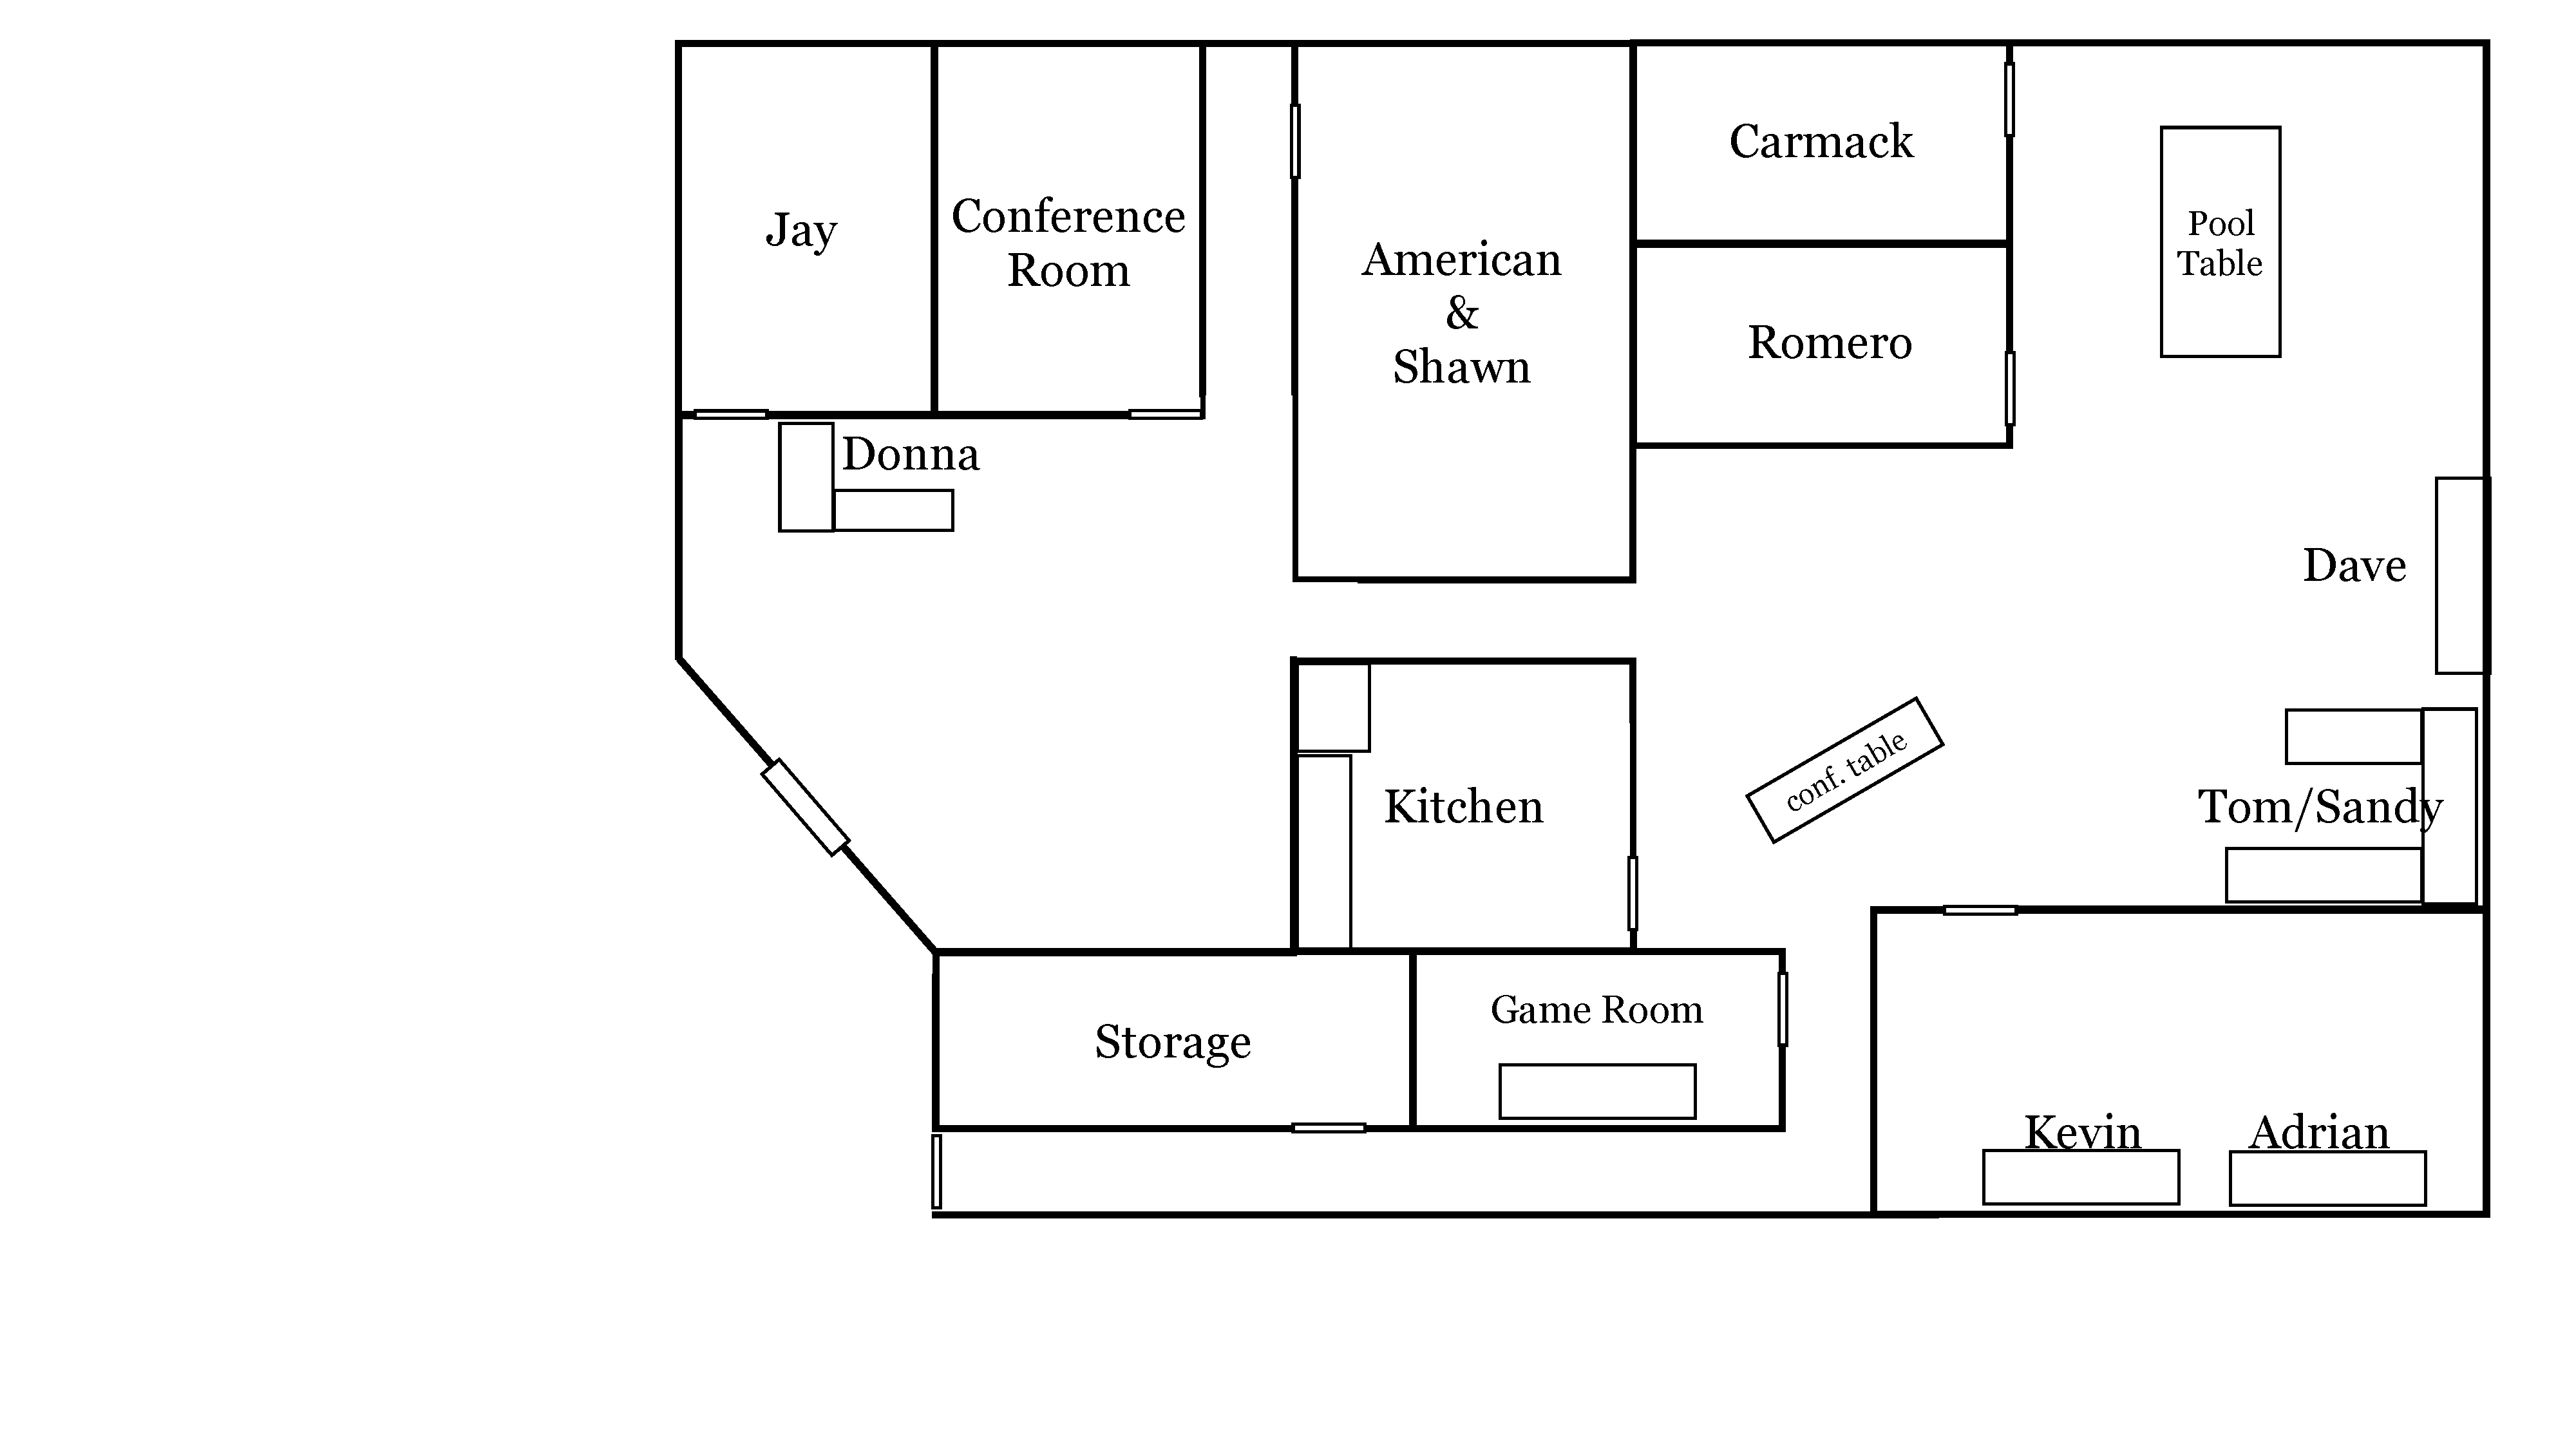
\includegraphics[width=\textwidth]{drawings/id-software-office-mesquite.pdf}
\caption{Id Software layout as it can be seen in John Romero mini documentary "A Visit to id Software (1993)".}
\end{figure}
\par
Dave Taylor memories are representative of id Software's unorthodox spirit at the time.\\
\par
\fq{I fell asleep on the floors a lot, which is why they got the sofa and had me test-drive it for comfort, but I only remember them taping my outline once. I believe it stuck around for a while though.}{Dave Taylor}\\
\par
\fq{I remember companies would send us free sound cards all the time, so many that we took to using them as ninja throwing stars at one point and would throw them into the kitchen wall opposite my desk.}{Dave Taylor}





\section{Creative direction}
The tone of the new title was to be much darker than the previous games. Initially intending to adapt the movie Aliens (1986) the team decided against it in order to retain total creative control\footnote{Amusingly, one of the best mod of all time would be the total conversion "Aliens TC.}. They wanted to do something scary, inspired by movie such as Evil Dead, The Thing, or The Fly and as aggressive as the metal music they usually listened to.\\
\par
Even the name of the next title would be to inspire fear. The idea would come from John Carmack while watching the movie "The color of money".\\ 
\par
Midway through the movie, Vincent played by Tom Cruise enters a pool bar carrying one of the best pool stick in the world, a Balabushka. Confident and commited on unleashing his skills upon his opponents. One of the local, Moselle, notices him entering. Intrigued by the pool cue case he asks Vincent: "What do you go in there?". "In Here?!" exclaims Vincent, looking up and smiling maliciously: "DOOM!".\\
\par

\par
\cfullimage{Doom_gibs.png}{"In Here ?......DOOM!"}
\par
The game they envisioned would go way beyond what they had accomplised with Wolfenstein 3D and Spear of Destiny. \doom~would have eight weapons and seventeen type of opponents. The hero would fight countless demons. And there would be a lots of gibs.

